\documentclass{beamer}
\usetheme{Madrid}

\title{The Kondo Problem: Numerical renormalization group and the single-impurity Anderson Model}
\subtitle{PHYS 4240: Solid State Physics}
\author{Casey Hampson}
\date{22 April, 2025}


\usepackage{amsmath}
\usepackage{amssymb}
\usepackage{siunitx}
\usepackage{mathtools}
\usepackage{esdiff}
\usepackage{esint}
\usepackage{bm}
\usepackage{tikz-feynman}
\usepackage{wrapfig}
\usepackage{braket}
\usepackage[utf8]{inputenc}

\newcommand{\dd}{\mathrm{d}}
\newcommand{\vv}[1]{\mathbf{\bm{#1}}}
\newcommand{\abs}[1]{\lvert #1 \rvert}

\usepackage[
backend=biber,
style=ieee
]{biblatex}
\addbibresource{./sources.bib}


\makeatletter
\pretocmd{\itemize}{\ifhmode\unvbox\voidb@x\fi}{}{}
\pretocmd{\enumerate}{\ifhmode\unvbox\voidb@x\fi}{}{}
\makeatother


\begin{document}
\frame{\titlepage}



\begin{frame}
  \frametitle{Introduction}

  \begin{itemize}
  \item In the 1930s, experiments revealed some interesting behavior in low-temperature measurements of the resistance of certain metals like Gold.
  \item The expectation was that the resistance decreases monotonically with temperature due to decreasing electron-phonon interactions.
  \item However, the observation was that a minimum was reached and the resistance started growing again at lower temperatures.
  \end{itemize}

  \begin{figure}
    \centering
    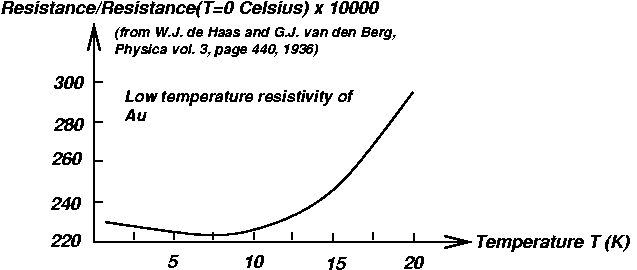
\includegraphics[width=0.6\textwidth]{./gfx/classickondo.png}
    \caption{Figure created using measurements found in~\cite{DeHaas_1936}.}
    \label{fig:classickondo}
  \end{figure}
  
\end{frame}


\begin{frame}
  \frametitle{Kondo's Solution}

  \begin{itemize}
  \item Eventually it became known that this was due to impurities within the metal.
  \item Jun Kondo then used perturbation theory on the spin-spin interaction between the impurity and the conduction electrons in the host metal:
    \begin{gather*}
      H = \sum_{\vv{k},\sigma} \epsilon_{\vv{k}}c^\dagger_{\vv{k},\sigma}c_{\vv{k},\sigma} + J\sum_{\vv{k},\vv{k}',\alpha,\beta} c^\dagger_{\vv{k},\alpha} \vv{\sigma}_{\alpha,\beta} c_{\vv{k}',\beta} \cdot \vv{S}.
    \end{gather*}
  \item This yielded corrections to the resistance that looked like
    \begin{gather*}
      R(T) = aT^5 + c_{\mathrm{imp}}R_0 - c_{\mathrm{imp}}R_1\log\left( \frac{k_B T}{D} \right).
    \end{gather*}
  \item Yielded correct behavior \textit{at} the minimum, but diverges for $T\rightarrow0$.
  \end{itemize}
\end{frame}


\begin{frame}
  \frametitle{Other Attempts at Solutions}

  \begin{itemize}
  \item After this, a number more models were introduced, one in particular being Anderson's \textit{Poor Man's Scaling} method~\cite{Anderson_1970}.
  \item This method was effectively a renormalization group approach, but again failed at low temperatures.
  \item This was because subsequent renormalizations increased $J$ to infinity, the parameter by which perturbation theory was applied later on.
  \item In 1975, Wilson~\cite{Wilson_1975} used the numerical renormalization group to approach the problem non-perturbatively, finally leading to accurate solutions in the low-energy regime.
  \end{itemize}
\end{frame}



\begin{frame}
  \frametitle{Poor Man's Scaling}
  
  \begin{figure}[ht!]
    \centering
    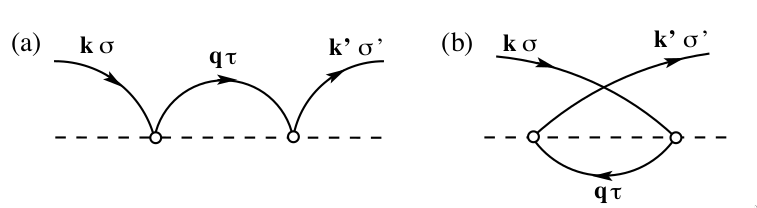
\includegraphics[width=0.5\textwidth]{./gfx/poormans-feynman.png}
  \end{figure}

  \begin{itemize}
  \item One approach to this method is considering the scattering between electrons from an initial state $\ket{\vv{k}}$ to a final $\ket{\vv{k}'}$.
  \item We consider the so-called scattering $T$-matrix:
    \begin{gather*}
      T_{\vv{k}',\vv{k}}(\omega) = V_{\vv{k}',\vv{k}} + V_{\vv{k}',\vv{q}} G_0(\omega,\vv{q})T(\omega)
    \end{gather*}
    where $V$ is the Kondo exchange interaction $V \propto J$.
  \item By calculating this to second order in $V$, we are effectively renormalizing the interaction:
    \begin{gather*}
      \hat{V} \rightarrow \hat{V}' = \hat{V} + \hat{V} \frac{1}{\omega - \hat{H}_0} \hat{V}
    \end{gather*}
  \end{itemize}
\end{frame}

\begin{frame}
  \frametitle{Poor Man's Scaling}

  \begin{itemize}
  \item After some derivations, what we find is that the renormalization of the interactions look like $J_\alpha \rightarrow J_\alpha + \delta J_\alpha$ ($\alpha=\pm,z$), with
    \begin{gather*}
      \delta J_z = -J_\pm^2 \rho \abs{\delta\Lambda} \left[ \frac{1}{\omega - \Lambda + \epsilon_k} \frac{1}{\omega - \Lambda + \epsilon_{k'}}\right], \\
      \delta J_\pm = -J_z J_\pm \rho \abs{\delta\Lambda} \left[ \frac{1}{\omega - \Lambda + \epsilon_k} \frac{1}{\omega - \Lambda + \epsilon_{k'}}\right]
    \end{gather*}
  \item Leading to renormalization flow equations that go like
    \begin{gather*}
      \diff{g_z}{\ln \Lambda} = -2g_\pm^2 + \mathcal{O}(g^3), \\
      \diff{g_\pm}{\ln \Lambda} = -2g_z g_\pm + \mathcal{O}(g^3)
    \end{gather*}
    where $g$s are dimensionless couplings.
  \end{itemize}
  
\end{frame}


\begin{frame}
  \frametitle{Variational Methods}

  \begin{itemize}
  \item Variational methods can give us further qualitative understanding.
  \item We consider a filled Fermi sea of conduction electrons and a singly occupied d-orbital from the impurity.
  \item If the spins of a conduction electron and the d-orbital electron are the same, there are no important interactions, but if they are anti-parallel, virtual excitations may occur.
  \item A trial wavefunction representing this state is give by
    \begin{gather*}
      \ket{\psi_0} = \left[ \alpha_0 + \sum_{k<k_F,\sigma} \alpha_{\vv{k}}c^\dagger_{d,\sigma}c_{\vv{k},\sigma} \right]\ket{0}
    \end{gather*}
  \item Importantly, this is representative of a singlet state formed between the d-orbital of the impurity and a conduction electron.
  \end{itemize}
\end{frame}

\begin{frame}
  \frametitle{Variational Methods}

  \begin{itemize}
  \item We now consider the variational energy functional
    \begin{gather*}
      \tilde{E}[\ket{\psi_0}] = \frac{\braket{\psi_0 | H | \psi_0}}{\braket{\psi_0 | \psi_0}},
    \end{gather*}
    where we are considering the single-impurity Anderson Hamiltonian:
    \begin{align*}
      H &= \epsilon_d n_d + U n_{d\uparrow}n_{d\downarrow} + \sum_{\vv{k},\sigma} \epsilon_{\vv{k},\sigma}c^\dagger_{\vv{k},\sigma}c_{\vv{k},\sigma} \\
        &+ \sum_{\vv{k},\sigma} \left(V_{\vv{k}} c^\dagger_{\vv{k},\sigma}d_\sigma + V^*_{\vv{k}}d^\dagger_\sigma c_{\vv{k},\sigma}\right).
    \end{align*}
  \item All energies are measured relative to the Fermi surface.
  \end{itemize}
\end{frame}

\begin{frame}
  \frametitle{Variational Methods}

  \begin{itemize}
  \item By plugging $H$ into the energy functional, we arrive at
    \begin{gather*}
      \tilde{E} = 2 \sum_{k<k_F} \frac{\abs{V_{\vv{k}}}^2}{\tilde{E} - \epsilon_d + \epsilon_{\vv{k}}}.
    \end{gather*}
  \item Defining the binding energy $\Delta_K = \tilde{E} - \epsilon_d$, we find:
    \begin{gather*}
      \epsilon_d +\Delta_K = 2 \sum_{k<k_F} \frac{\abs{V_{\vv{k}}}^2}{\Delta_K - \abs{\epsilon_{\vv{k}}}}.
    \end{gather*}
  \item Converting to the continuum and letting $V_\vv{k} \rightarrow V$ (indep. of $\vv{k}$):
    \begin{gather*}
      \epsilon_d + \Delta_K = 2\rho\int_0^{\epsilon_F} \dd\epsilon \; \frac{-V^2}{\epsilon - \Delta_K} = -2\epsilon\abs{V}^2 \ln\left( \frac{\epsilon_F}{\abs{\Delta_K}} \right).
    \end{gather*}
  \end{itemize}
\end{frame}

\begin{frame}
  \frametitle{Variational Methods}

  \begin{itemize}
  \item When the energy of the d-level (relative to the Fermi surface) is much larger than the binding energy, we find
    \begin{gather*}
      \Delta_K = -\epsilon_F \exp\left[ -\frac{1}{2\rho J} \right],
    \end{gather*}
    where $J = V^2/\epsilon_d$ is defined as the coupling constant.
  \item Importantly, this is negative, indicating that the singlet state (represented by our original trial wavefunction) is the preferable and therefore likely state for this configuration.
  \end{itemize}
\end{frame}

\begin{frame}
  \frametitle{Kondo Resonance}

  \begin{itemize}
  \item We would expect, in the case of strong d-level on-site repulsion $U$, that $\braket{n_d} \approx 1$, or $1 - \braket{n_d} \approx 0$. What we find is
    \begin{gather*}
      1 - \braket{n_d} \approx \frac{\pi \Delta_K}{2\Delta} \ll 1 \neq 0
    \end{gather*}
  \item Because of a slightly less than unity d-level occupation, there is an excess of states in the Fermi surface.
  \item This observed increase in the density of states is what is called a \textbf{Kondo resonance}
  \end{itemize}

  \begin{figure}
    \centering
    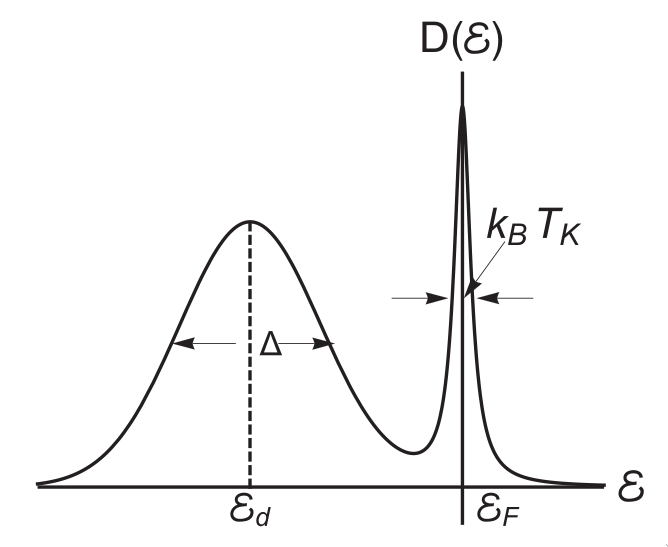
\includegraphics[width=0.4\linewidth]{./gfx/kondo-resonance.png}
  \end{figure}
\end{frame}

\begin{frame}
  \frametitle{Kondo Resonance}

  \begin{itemize}
  \item This leads often to the picture of what is called the \textbf{Kondo cloud}
  \end{itemize}

  \begin{figure}
    \centering
    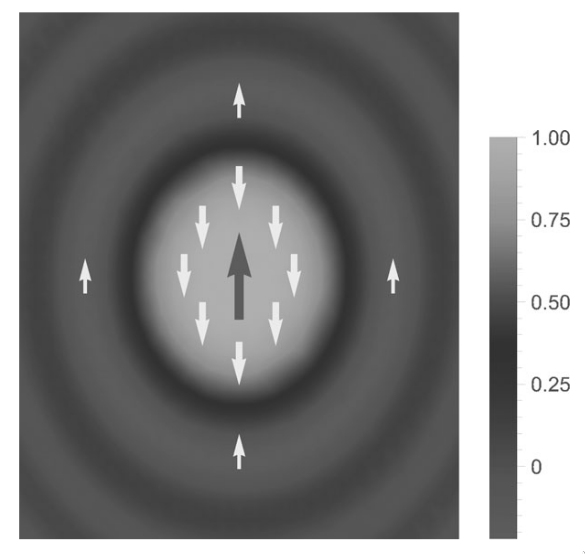
\includegraphics[width=0.3\linewidth]{./gfx/kondo-cloud.png}
  \end{figure}

  \begin{itemize}
  \item Due to the increased density of states, there is also an increase (a maximum is achieved) for the scattering probability between the d-level impurity states and the conduction electrons.
  \item This manifests in the observation of increasing resistivity as $T \rightarrow 0$.
  \end{itemize}
\end{frame}


\begin{frame}
  \frametitle{The Renormalization Group}

  \begin{itemize}
  \item The renormalization group is a mapping of a Hamiltonian $H(\vv{K})$ with a set of parameters $\vv{K}$ to another with parameters $\vv{K}'$, valid at a new energy scale.
    \begin{gather*}
      \mathcal{R}_\alpha [H(\vv{K})] = H(\vv{K}'),\quad\text{or}\quad \mathcal{R}_\alpha(\vv{K}) = \vv{K}'.
    \end{gather*}
  \item The parameter $\alpha$ is the ratio of the energy scales; characterizes the ``strength'' of the transformation.
  \item Subsequent transformations form a \textit{trajectory} in parameter space.
  \end{itemize}
\end{frame}

\begin{frame}
  \frametitle{Fixed Points}

  \begin{itemize}
  \item A \textbf{fixed point} is a set of params $\vv{K}^*$ that is invariant under the transformation:
    \begin{gather*}
      \mathcal{R}(\vv{K}^*) = \vv{K}^*.
    \end{gather*}
  \item We can linearize the transformation around this fixed point:
    \begin{gather*}
      \mathcal{R}_\alpha(\vv{K}^* + \delta\vv{K}) = \vv{K}^* + \vv{L}^*_\alpha \delta\vv{K} + \mathcal{O}(\delta\vv{K}^2),
    \end{gather*}
  \item Then we can express the mapping in terms of the eigenvectors/eigenvalues of $\vv{L}^*_\alpha$:
    \begin{gather*}
      \mathcal{R}^m_\alpha(\vv{K}^* + \delta\vv{K}) = \vv{K}^* + \sum_n (\delta K)_n(\lambda^*_n)^m \vv{V}^*_n.
    \end{gather*}
  \end{itemize}
\end{frame}


\begin{frame}
  \frametitle{Fixed Points}

  \begin{itemize}
  \item The point of doing this is so that we are able to effectively describe behavior \textit{around} a fixed point using the effective Hamiltonian at that fixed point.
  \item We can make the connection from poor man's scaling results that the $J \rightarrow \infty$ / $T \rightarrow 0$ point is a fixed point.
  \item What we want to do is formalize our renormalization group transformations and determine the effective Hamiltonian for the $J \rightarrow \infty$ fixed point.
  \item We are then able to describe the behavior around the fixed point with this effective Hamiltonian and determine important quantities.
  \item In the trajectories/flows of our parameters, we also are able to recognize the transitions between fixed points.
  \end{itemize}
\end{frame}




\begin{frame}
  \frametitle{The Numerical Renormalization Group (NRG)}

  The NRG is highly specialized per problem, but generally follows these steps:

  \begin{figure}
    \centering
    \includegraphics<1>[width=0.4\textwidth]{./gfx/nrg-a.png}
    \includegraphics<2>[width=0.4\textwidth]{./gfx/nrg-b.png}
    \includegraphics<3>[width=0.4\textwidth]{./gfx/nrg-c.png}
    \includegraphics<4>[width=0.4\textwidth]{./gfx/nrg-c.png}
  \end{figure}
  
  \begin{enumerate}
  \item Divide the energy spectrum into logarithmic bins via a parameter $\Lambda>1$: we get intervals $[\Lambda^{-(n+1)},\Lambda^{-n}]$, $[-\Lambda^{-n},\Lambda^{-(n+1)}]$.
    \pause
  \item Pick a single characteristic state from each interval.
    \pause
  \item Map these discrete states onto a semi-infinite chain, with the impurity placed at one end.
    \pause
  \item Iteratively diagonalize the resulting Hamiltonian, adding a site each iteration.
  \end{enumerate}
\end{frame}


\begin{frame}
  \frametitle{The NRG}

  \begin{itemize}
  \item By logarithmically discretizing the energy spectrum, we arrive at the following relation for the hopping terms:
    \begin{gather*}
      t_n = \Lambda^{-n/2} \frac{(1+\Lambda^{-1})(1-\Lambda^{-n-1})}{2\sqrt{1-\Lambda^{-2n-1}}\sqrt{1-\Lambda^{-2n-3}}}.
    \end{gather*}
  \item We notice $t_n \propto 1/\sqrt{\Lambda}$, meaning that adding a term corresponds to accessing a new energy scale that is reduced by a factor of $\sqrt{\Lambda}$.
  \item This is the essence of the NRG.
  \end{itemize}
\end{frame}

\begin{frame}
  \frametitle{Single-Impurity Anderson Model (SIAM)}

  \begin{itemize}
  \item The SIAM considers that the impurity is represented by local moment formed via the Coulomb interaction $U$ between the two electrons in the state.
    \begin{gather*}
      H = \sum_\sigma \epsilon_d d^\dagger_\sigma d_\sigma + Ud^\dagger_\uparrow d_\uparrow d^\dagger_\downarrow d_\downarrow + \sum_{k,\sigma} \epsilon_k c^\dagger_{k,\sigma}c_{k,\sigma} + \sum_{k,\sigma} V_k(d^\dagger_\sigma c_{k,\sigma} + \mathrm{h.c.}).
    \end{gather*}
  \item The $d$s are creation/annihilation operators for impurity states, $c$s are for conduction states, and $V$ is the hybridization term.
  \end{itemize}
\end{frame}

\begin{frame}
  \frametitle{Logarithmic Discretization}

  \begin{itemize}
  \item Can bring the Hamiltonian to a quasi-continuous one:
    \begin{gather*}
      H = H_{\mathrm{imp}} + \sum_\sigma \int_{-1}^1 \dd\epsilon \; g(\epsilon) a^\dagger_{\epsilon,\sigma}a_{\epsilon,\sigma} + \sum_\sigma \int_{-1}^1 \dd\epsilon \; h(\epsilon) (d^\dagger_\sigma a_{\epsilon,\sigma} + \mathrm{h.c.}).
    \end{gather*}
  \item These new operators satisfy the standard fermionic anti-commutation relations:
    \begin{gather*}
      \{ a^\dagger_{\epsilon,\sigma},a_{\epsilon'\sigma'} \} = \delta(\epsilon-\epsilon')\delta_{\sigma,\sigma'}.
    \end{gather*}
  \item We can then discretize the model with points $x_n = \pm \Lambda^{-n}$, where $n =0,1,2,\ldots$ and $\Lambda > 1$.
  \end{itemize}
\end{frame}

\begin{frame}
  \frametitle{Logarithmic Discretization}

  \begin{itemize}
  \item Inside each iterval, we define a new basis which are simply plane waves:
    \begin{gather*}
      \psi^{\pm}_{np}(\epsilon) =
      \begin{alignedat}{1}
        \begin{cases}
          \frac{1}{\sqrt{d_n}}e^{\pm i\omega_n p\epsilon}, \quad & \text{for}\ x_{n+1} < \epsilon < x_n,\ \text{and} \\
          0 & \text{otherwise}.
        \end{cases}
      \end{alignedat}
    \end{gather*}
    where $p \in \mathbb{Z}$ and $\omega_n = 2\pi/d_n$ is the characteristic frequency.
  \item Expanding our continuous $a$ operators in terms of these (simply a Fourier expansion) we find:
    \begin{gather*}
      a_{\epsilon\sigma} = \sum_{np} (a_{np\sigma}\psi^+_{np}(\epsilon) + b_{np\sigma}\psi^-_{np}(\epsilon))
    \end{gather*}
  \item Using these, our quasi-continuous Hamiltonian is now expanded in terms of logarithmically discretized creation/annihilation operators.
  \end{itemize}
\end{frame}



\begin{frame}
  \frametitle{Mapping to semi-infinite chain}

  \begin{itemize}
  \item With the Hamiltonian now logarithmically discretized, one can follow a tridiagonalization procedure in order to put it in the form of the semi-infinite chain (tight-binding form):
    \begin{align*}
      H = H_{\mathrm{imp}} &+ \sqrt{\frac{\xi_0}{\pi}}\sum_\sigma (f^\dagger_\sigma c_{0,\sigma} + c^\dagger_{0,\sigma}f_\sigma) \\
      &+ \sum_{\sigma,n=0}^{\infty} \left[ \epsilon_n c^\dagger_{n,\sigma}c_{n,\sigma} + t_n(c^\dagger_{n,\sigma}c_{n+1,\sigma} + c^\dagger_{n+1,\sigma}c_{n,\sigma}) \right].
    \end{align*}
  \item Assuming a particle-hole symmetric hybridization $\Delta(\omega) = \Delta(-\omega)$ and a $k$-independent hybridization term $V$, we have that $\epsilon_n = 0$ and $\sqrt{\xi_0/\pi} \rightarrow V$:
    \begin{align*}
      H = \epsilon_d n_d + Un_{d\uparrow}n_{d\downarrow} &+ V\sum_\sigma (d^\dagger_\sigma c_{0,\sigma} + c^\dagger_{0,\sigma} d_\sigma) \\
      &+ \sum_{\sigma,n=0}^{\infty} \left[t_n(c^\dagger_{n,\sigma}c_{n+1,\sigma} + c^\dagger_{n+1,\sigma}c_{n,\sigma}) \right].
    \end{align*}
  \end{itemize}
\end{frame}



\begin{frame}
  \frametitle{Connection to the Renormalization Group}

  \begin{itemize}
  \item Due to the choice of logarithmic binning, Wilson~\cite{Wilson_1975} calculated that the hopping terms decrease exponentially:
    \begin{gather*}
      t_n = \Lambda^{-n/2}\frac{(1 + \Lambda^{-1})(1 - \Lambda^{-n-1})}{2\sqrt{1 - \Lambda^{-2n-1}}\sqrt{1 - \Lambda^{-2n-3}}}.
    \end{gather*}
  \item Therefore, what we are doing by adding a site to the infinite chain is accessing an energy scale that is decreased by a factor of $\sqrt{\Lambda}$.
  \item In particular, we consider the main chain Hamiltonian is the limit of a sequence of Hamiltonians parameterized by $N$ such that
    \begin{gather*}
      H = \lim_{N\rightarrow\infty} \Lambda^{-(N-1)/2}H_N,
    \end{gather*}
    where
    \begin{align*}
      H_N = \Lambda^{(N-1)/2} &\big[ H_{\mathrm{imp}} + V\sum_\sigma (f^\dagger_\sigma c_{0,\sigma} + c^\dagger_{0,\sigma}f_\sigma)\\
                              &+ \sum_{\sigma,n=0}^{N-1} t_n(c^\dagger_{n,\sigma}c_{n+1,\sigma} + c^\dagger_{n+1,\sigma}c_{n,\sigma}) \big].
    \end{align*}
  \end{itemize}
\end{frame}

\begin{frame}
  \frametitle{Connection to the Renormalization Group}

  \begin{itemize}
  \item With this definition, we define recursion relations for subsequent Hamiltonians:
    \begin{gather*}
      H_{N+1} = \sqrt{\Lambda}H_N + \Lambda^{N/2}\sum_\sigma t_N (c^\dagger_{N,\sigma}c_{N+1,\sigma} + c^\dagger_{N+1,\sigma}c_{N,\sigma}),
    \end{gather*}
    with the initial given by
    \begin{gather*}
      H_0 = \Lambda^{-1/2}\left[ \sum_\sigma \epsilon_f f^\dagger_\sigma f_\sigma + Uf^\dagger_\uparrow f_\uparrow f^\dagger_\downarrow f_\downarrow + V\sum_\sigma (f^\dagger_\sigma c_{0,\sigma} + c^\dagger_{0,\sigma}f_\sigma) \right].
    \end{gather*}
  \item Therefore, what we have when going to $H_N$ to $H_{N+1}$ is a renormalization group transformation: $\mathcal{R}_\alpha[H_{N}] = H_{N+1}$, with $\alpha$ parameterized via $\sqrt{\Lambda}$.
  \end{itemize}
\end{frame}


\begin{frame}
  \frametitle{Iterative diagonalization of the semi-infinite chain}

  \begin{itemize}
  \item As described, the procedure from here involves repeatedly adding sites to the chain and diagonalizing the resulting Hamiltonian.
  \item Due to the choice of basis, the dimensionality of the Hamiltonian increases exponentially each iteration.
  \item By sorting the energies and truncating them to keep only some fixed $N_s$ lowest-lying energies, we remove the higher energy terms which have decreasing effect on the low energy behavior of the system.
  \end{itemize}

  \begin{figure}
    \centering
    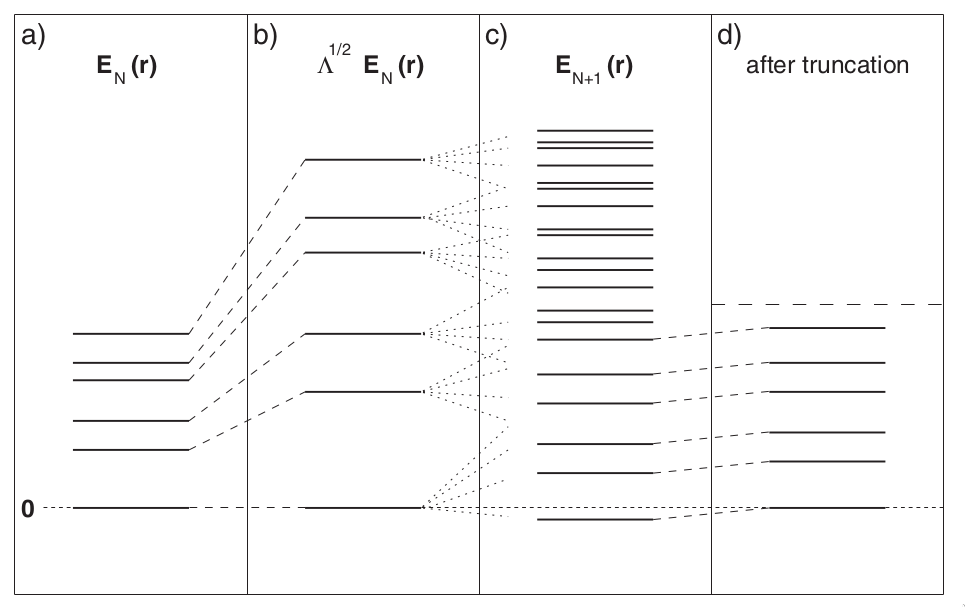
\includegraphics[width=0.5\textwidth]{./gfx/truncation.png}
  \end{figure}
\end{frame}

\begin{frame}
  \frametitle{Iterative diagonalization of the semi-infinite chain}

  \begin{itemize}
  \item For this problem, we choose our basis to be the Fock basis consisting of four states: $\ket{0}$, $\ket{\uparrow}$, $\ket{\downarrow}$, and $\ket{\uparrow\downarrow}$ related to empty, single, or doubly-occupied states.
  \item Each iteration, we construct a new basis that is the outer product of the original bases $\ket{r}_N$ and the new basis $\ket{s_{n+1}}$.
  \end{itemize}

  \begin{figure}
    \centering
    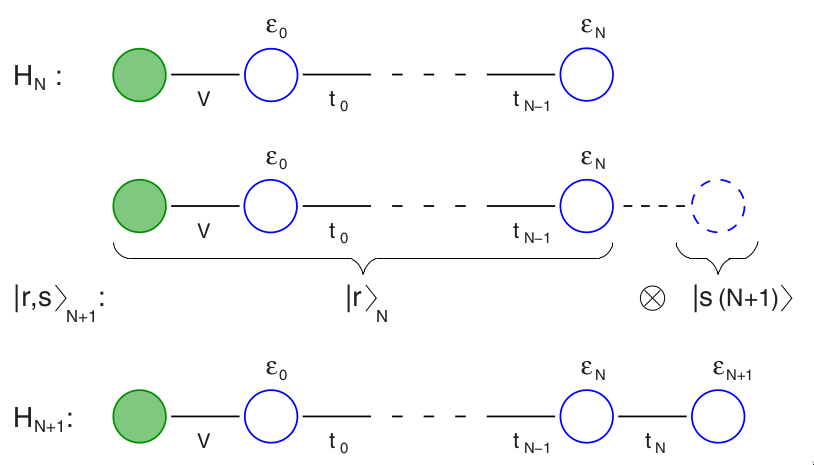
\includegraphics[width=0.6\textwidth]{./gfx/outer-product.png}
  \end{figure}
\end{frame}


\begin{frame}
  \frametitle{Initial iteration}

  \begin{itemize}
  \item For the initial iteration, we start by considering just the impurity and one conduction site; can construct the Hamiltonian in the combined Fock basis like so:
    \begin{gather*}
      H = I_4 \otimes H_{\mathrm{imp}} + H_{\mathrm{hyb}}, \\
      H_{\mathrm{hyb}} = V\sum_\sigma (c^\dagger_{0,\sigma} \otimes f_\sigma + c_{0,\sigma} \otimes f^\dagger_\sigma).
    \end{gather*}
  \item With our choice of basis, we consider the form of the creation and annihilation operators ($c$s and $f$s are identical):
    \begin{gather*}
      f^\dagger_\uparrow =
      \begin{pmatrix}0 & 0 & 0 & 0 \\ 1 & 0 & 0 & 0 \\ 0 & 0 & 0 & 0 \\ 0 & 0 & -1 & 0\end{pmatrix},\quad f^\dagger_\downarrow =
      \begin{pmatrix}0 & 0 & 0 & 0 \\ 0 & 0 & 0 & 0 \\ 1 & 0 & 0 & 0 \\ 0 & 1 & 0 & 0\end{pmatrix}
    \end{gather*}
  \item The $-1$ is due to the fermionic nature of the operators.
  \end{itemize}
\end{frame}

\begin{frame}
  \frametitle{Initial iteration}

  \begin{itemize}
  \item With this, we are able to construct the (symmetrized) initial Hamiltonian
    \begin{gather*}
      H_0 =
      \begin{pmatrix}
        \mathcal{H}_{\mathrm{imp}} & Vf_\uparrow & Vf_\downarrow & 0 \\
        Vf^\dagger_\uparrow & \mathcal{H}_{\mathrm{imp}} & 0 & Vf_\downarrow \\
        Vf^\dagger_\downarrow & 0 & \mathcal{H}_{\mathrm{imp}} & -Vf_\uparrow \\
        0 & Vf^\dagger_\downarrow & -Vf^\dagger_\uparrow & \mathcal{H}_{\mathrm{imp}}
      \end{pmatrix}
    \end{gather*}
    where $\mathcal{H}_{\mathrm{imp}}$ represents the impurity occupation energies acting on the impurity subspace:
    \begin{gather*}
      \mathcal{H}_{\mathrm{imp}} =
      \begin{pmatrix}0 & 0 & 0 & 0 \\  0 & \epsilon_f & 0 & 0 \\ 0 & 0 & \epsilon_f & 0 \\ 0 & 0 & 0 & 2\epsilon_f + U\end{pmatrix}
    \end{gather*}
  \end{itemize}
\end{frame}

\begin{frame}
  \frametitle{Symmetries}

  \begin{itemize}
  \item As mentioned before, the dimensionality of this Hamiltonian rapidly approaches being unfeasible to diagonalize.
  \item We can utilize symmetries, in particular $S_z$ (twice the $z$-component of spin) and $Q$ (charge with respect to half-filling)
    \begin{gather*}
      S_z \rightarrow [0,1,-1,0], \quad Q \rightarrow [-1,0,0,1]
    \end{gather*}
  \item Since these are good quantum numbers, we can construct an operator combining them that commutes with the Hamiltonian.
  \item This effectively reduces the single matrix into several (significantly) smaller matrices corresponding to the states with the same eigenvalue of the new operator.
  \end{itemize}
\end{frame}

\begin{frame}
  \frametitle{Subsequent Iterations}

  \begin{itemize}
  \item Subsequent iterations increase the dimensionality by 4, but the structure of placing identities and the creation and annihilation operators remains largely the same, but instead with $t_n$s for the hopping parts.
    \begin{gather*}
      t_n (c^\dagger_{n+1,\sigma} \otimes c_{n,\sigma} + c_{n+1,\sigma} \otimes c^\dagger_{n,\sigma})
    \end{gather*}
  \item The diagonals are then the energies from the previous iteration.
  \item If $N > N_s$, we truncate the highest energy parts and keep the remaining $N_s$ states.
  \item The energies are ordered and thus are the states, so we must rotate the operators:
    \begin{gather*}
      f^\dagger_\sigma \rightarrow \vv{C}_n^\intercal f^\dagger_\sigma \vv{C}_n
    \end{gather*}
  \item We also calculate thermodynamic quantities.
  \end{itemize}
\end{frame}


\begin{frame}
  \frametitle{Calculation of Physical Quantities}

  \begin{itemize}
  \item Each added site/iteration corresponds to a temperature $T_N$:
    \begin{gather*}
      k_B T_N = \frac{1}{2}(1 + \Lambda^{-1})\Lambda^{-(N-1)/2}/\bar{\beta}.
    \end{gather*}
  \item It turns out we can choose $\bar{\beta}$ to be in the range 0.5 to 1, from which we calculate the temperature for that particular iteration.
  \item This is because when evaluating things like the partition function, a low $\beta$ requires higher energy terms, which we drop from the truncation scheme, and a higher $\beta$ simply involves fewer terms leading to less accuracy.
  \item For each iteration, we determine this temperature, then determine additional physical quantities.
  \end{itemize}
\end{frame}

\begin{frame}
  \frametitle{Calculation of Physical Quantities}

  \begin{itemize}
  \item After determining the temperature, we can find the entropy, specific heat, and susceptibility:
    \begin{gather*}
      S = \beta\braket{H} + \ln Z, \\
      C = \beta^2(\braket{H^2} - \braket{H}^2), \\
      \chi_{\mathrm{tot}} =\beta(\braket{S_{\mathrm{tot},z}^2} - \braket{S_{\mathrm{tot},z}}^2).
    \end{gather*}
  \item Here, the average of a quantity $X$ is given by
    \begin{gather*}
      \braket{X} = \frac{1}{Z} \sum_i X_i e^{-\beta X_i},
    \end{gather*}
    with $Z$ being the standard partition function.
  \item To get the contributions to these values of the impurity only, we subtract off from this value with the impurity the result from a simple fermionic chain (without the impurity).
  \end{itemize}
\end{frame}

\begin{frame}
  \frametitle{Energy Flows \\ $N_s=1000$, $\Lambda$=3.0, $N=70$ \\ $\epsilon_f=\num{-0.5d-4}$, $U=\num{-e3}$, $V=\num{4d-4}$}

  \begin{figure}
    \centering
    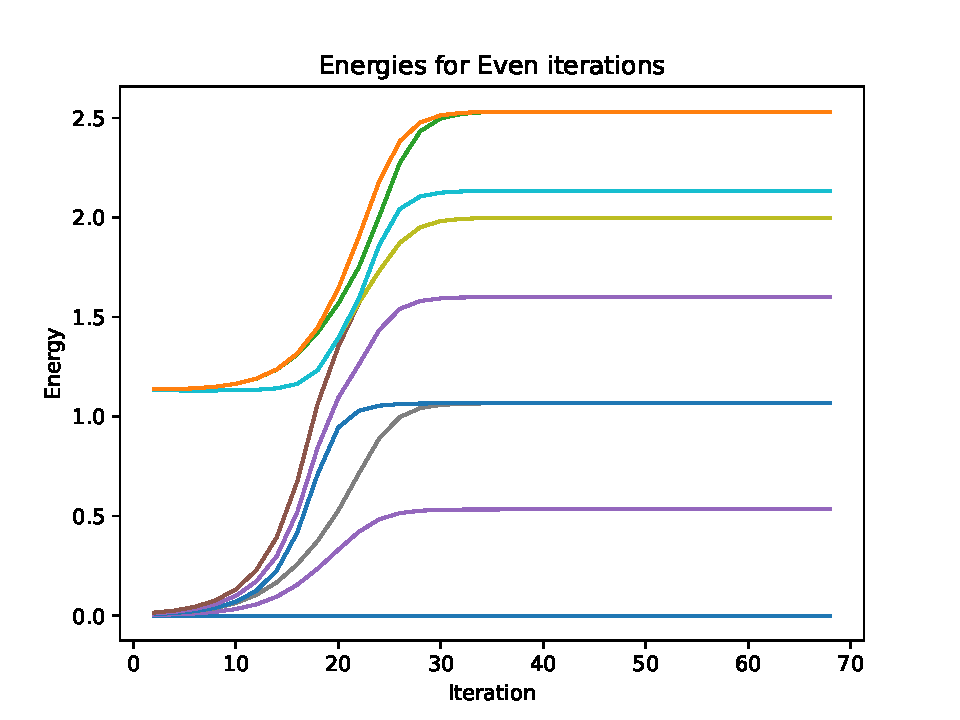
\includegraphics[width=0.49\linewidth]{./gfx/even_lowU.pdf}
    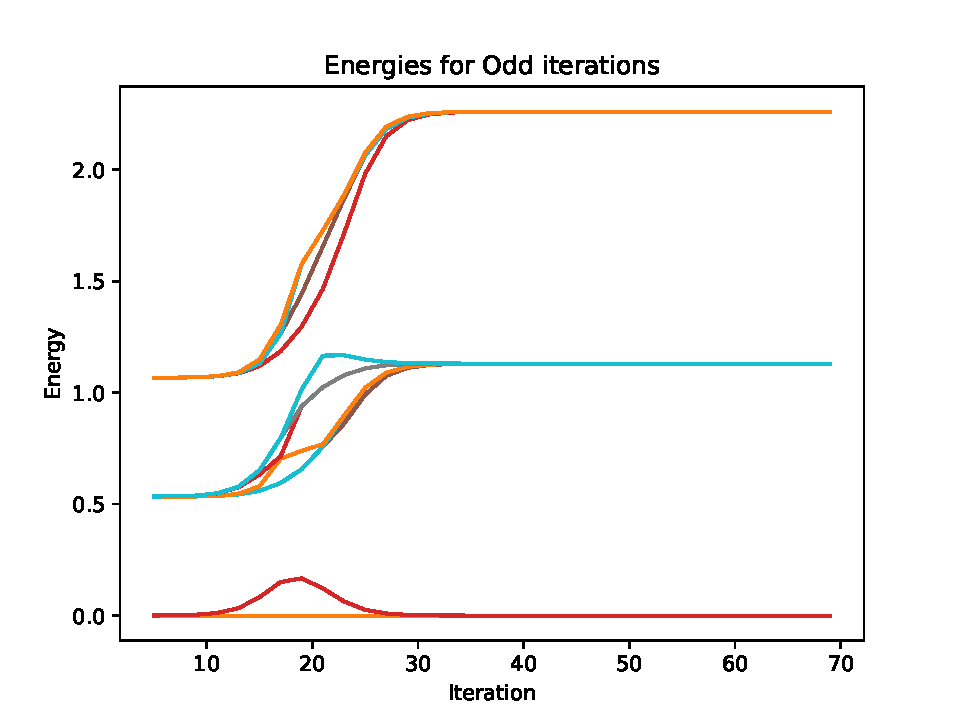
\includegraphics[width=0.49\linewidth]{./gfx/odd_lowU.pdf}
  \end{figure}

  \begin{itemize}
  \item We immediately notice that there is a crossover after a few iterations: this corresponds to the crossover between the $T \gg T_K$ fixed point and the $T \sim T_K$ fixed point, corresponding to a free moment and the strongly-coupled Kondo singlet
  \end{itemize}
\end{frame}

\begin{frame}
  \frametitle{Energy Flows \\ $N_s=1000$, $\Lambda$=3.0, $N=70$ \\ $\epsilon_f=\num{-0.5d-3}$, $U=\num{-e2}$, $V=\num{4d-4}$}

  \begin{itemize}
  \item Increasing $U$ (and $\epsilon_d$) by 10, we find that there is an intermediate fixed point corresponding to a weak coupling between a local moment and the conduction electrons.
  \end{itemize}

  \begin{figure}
    \centering
    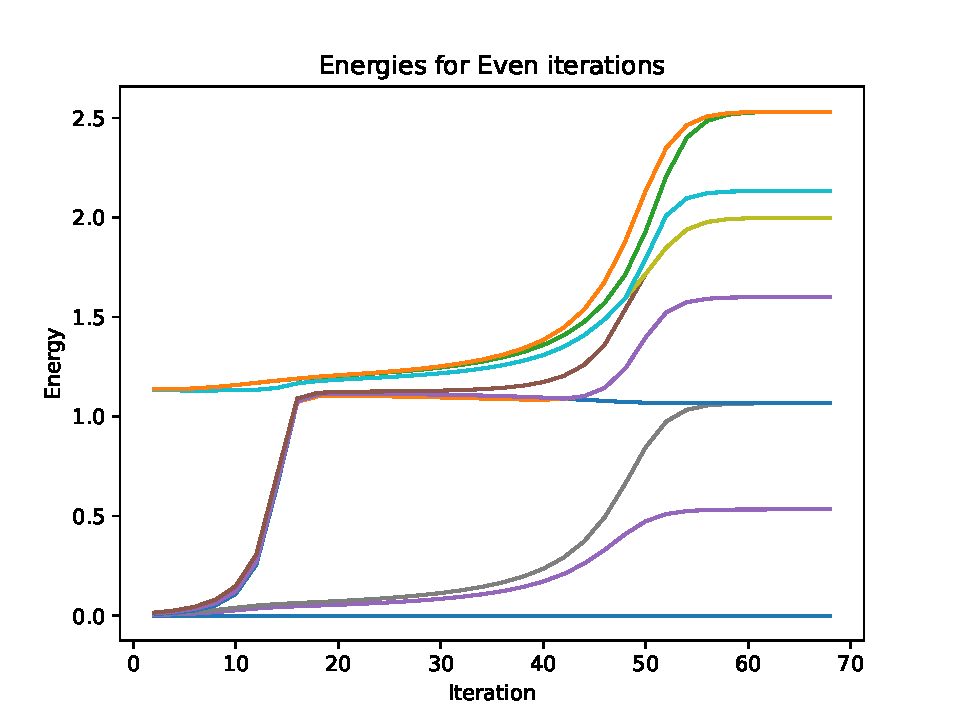
\includegraphics[width=0.49\linewidth]{./gfx/even.pdf}
    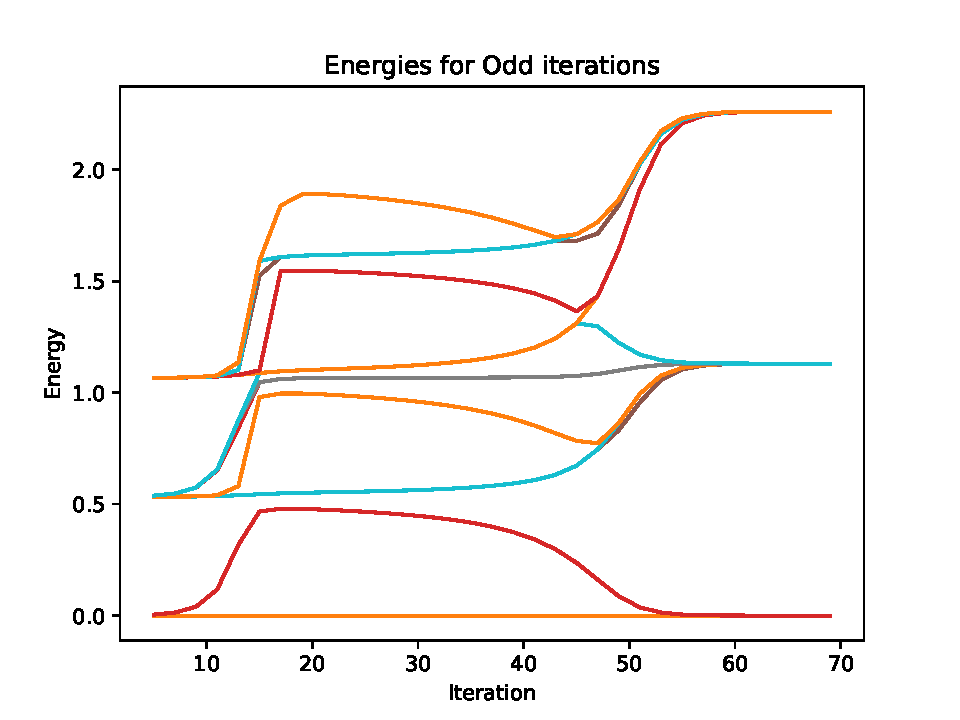
\includegraphics[width=0.49\linewidth]{./gfx/odd.pdf}
  \end{figure}
\end{frame}

\begin{frame}
  \frametitle{Existing Results}

  \begin{itemize}
  \item Some results were hard to directly compare; things like choice of $\bar{\beta}$ weren't clear from papers
  \end{itemize}

  \begin{figure}
    \centering
    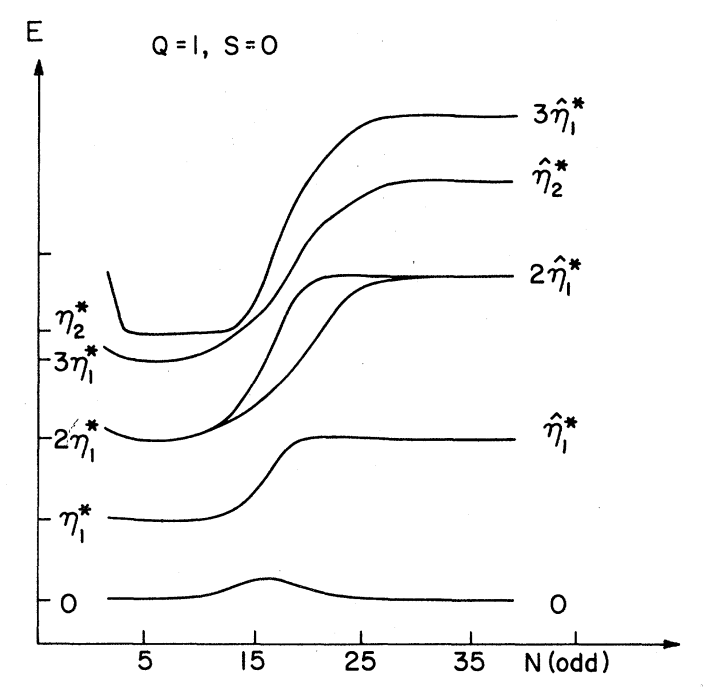
\includegraphics[width=0.49\linewidth]{./gfx/krishna-murthy-energies.png}
    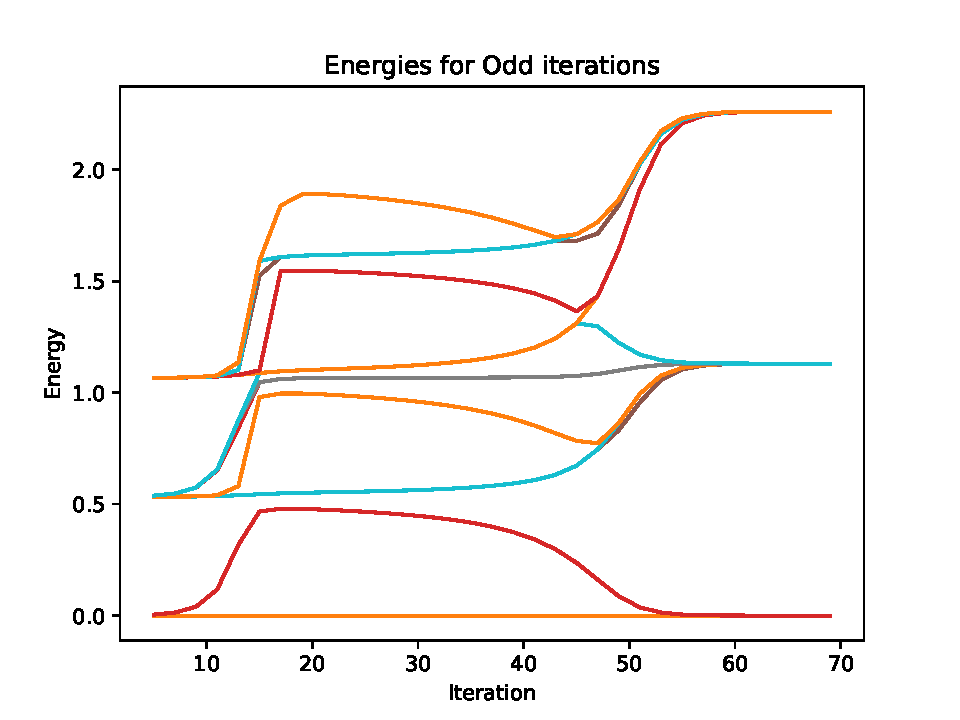
\includegraphics[width=0.49\linewidth]{./gfx/odd.pdf}
    \caption{Left is from~\cite{Krishna-murthy_Wilkins_Wilson_1980}.}
  \end{figure}
\end{frame}

\begin{frame}
  \frametitle{Impurity Contribution to Magnetic Susceptibility}

  \begin{itemize}
  \item The form of the susceptibility is as follows:
    \begin{align*}
      \chi_{\mathrm{imp}}(T) &= \frac{(g\mu_B)^2}{4k_BT[1 + \exp(-U/2k_BT)]} \quad\text{with}\ g\mu_B \rightarrow 1, \\
      4k_BT\chi_{\mathrm{imp}} &= \frac{1}{1 + e^{-U/2k_BT}}.
    \end{align*}
  \item If we take the onsite repulsion term $U$ to be small enough, there is only one crossover region between two fixed points: the free moment and the strongly coupled Kondo singlet.
  \item From the above expression, we expect the free moment ($T \gg U$) to have $4k_BT\chi_{\mathrm{imp}} = 1/8$.
  \item In the strong coupling limit, though, we expect for the local moment's spin to be entirely screened/compensated, giving no net addition to the susceptibility.
  \end{itemize}
\end{frame}

\begin{frame}
  \frametitle{Impurity Contribution to Magnetic Susceptibility}

  \begin{figure}
    \centering
    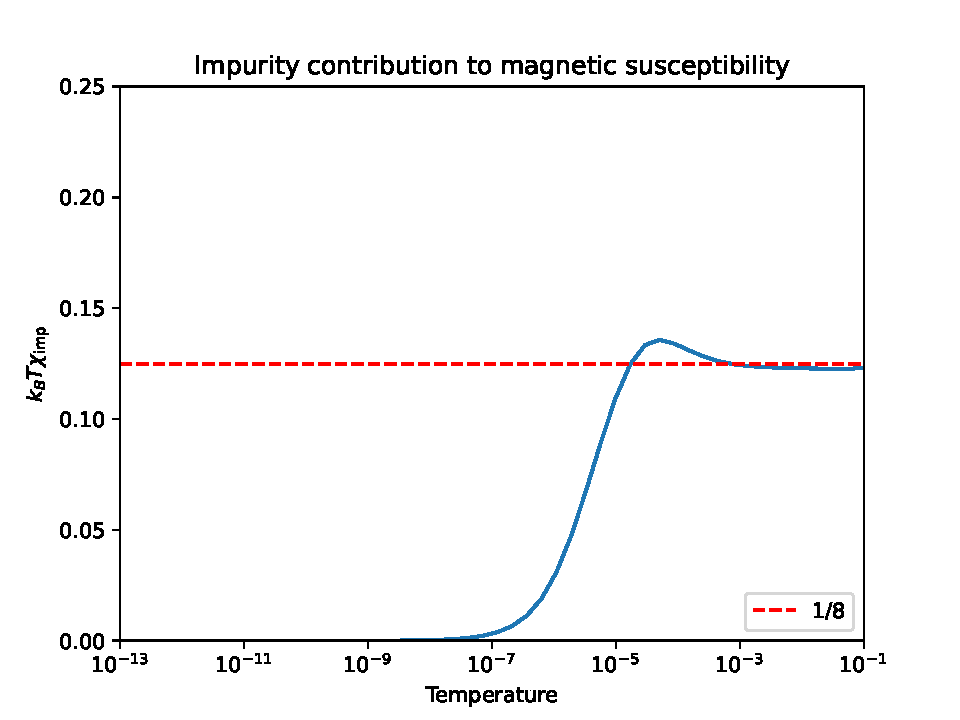
\includegraphics[width=0.75\linewidth]{./gfx/tchi_lowU.pdf}
  \end{figure}
\end{frame}

\begin{frame}
  \frametitle{Impurity Contribution to Magnetic Susceptibility}

  \begin{itemize}
  \item However, we can also have a case with a strong onsite repulsion $U$, in which there is an intermediate region characterized by a local moment weakly coupled to the conduction electrons.
  \item From the previous equation we would expect, for this region, that $4k_BT\chi_{\mathrm{imp}} \approx 1/4$:
  \end{itemize}

  \begin{figure}
    \centering
    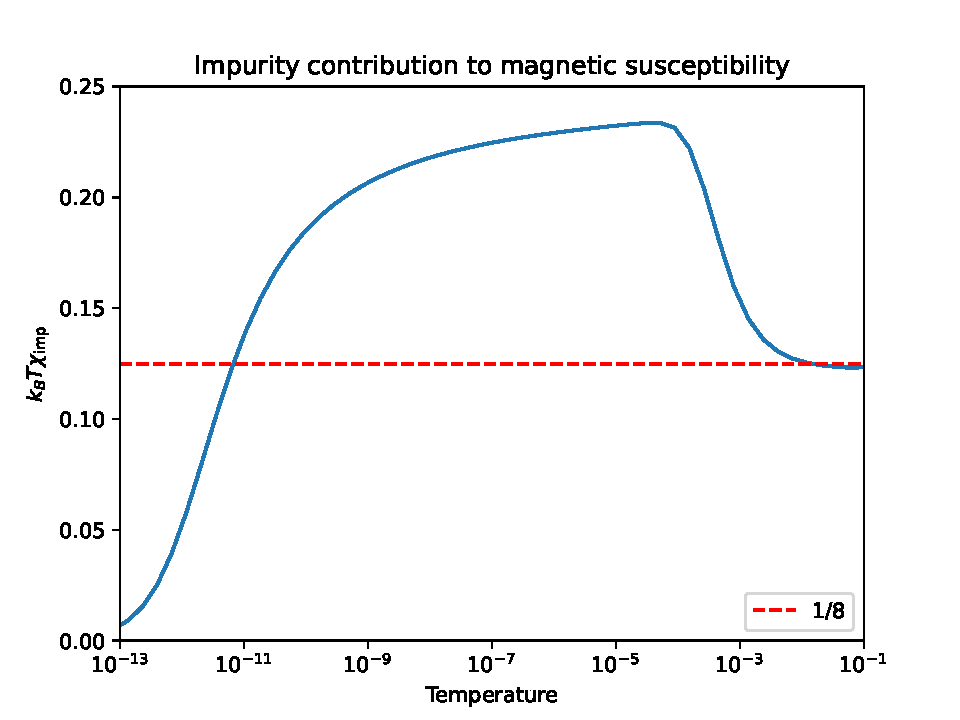
\includegraphics[width=0.6\linewidth]{./gfx/tchi.pdf}
  \end{figure}
\end{frame}

\begin{frame}
  \frametitle{Impurity Contribution to Entropy}

  \begin{itemize}
  \item Entropy is related to the logarithm of the multiplicity: $S = k_B \ln\Omega$.
  \item For the small $U$ case, the Kondo singlet has a multiplicity of unity: $S = 0$, but in the free limit, the multiplicity is 2, leading to ordinary $S = k_B\ln2$ behavior.
  \end{itemize}

  \begin{figure}
    \centering
    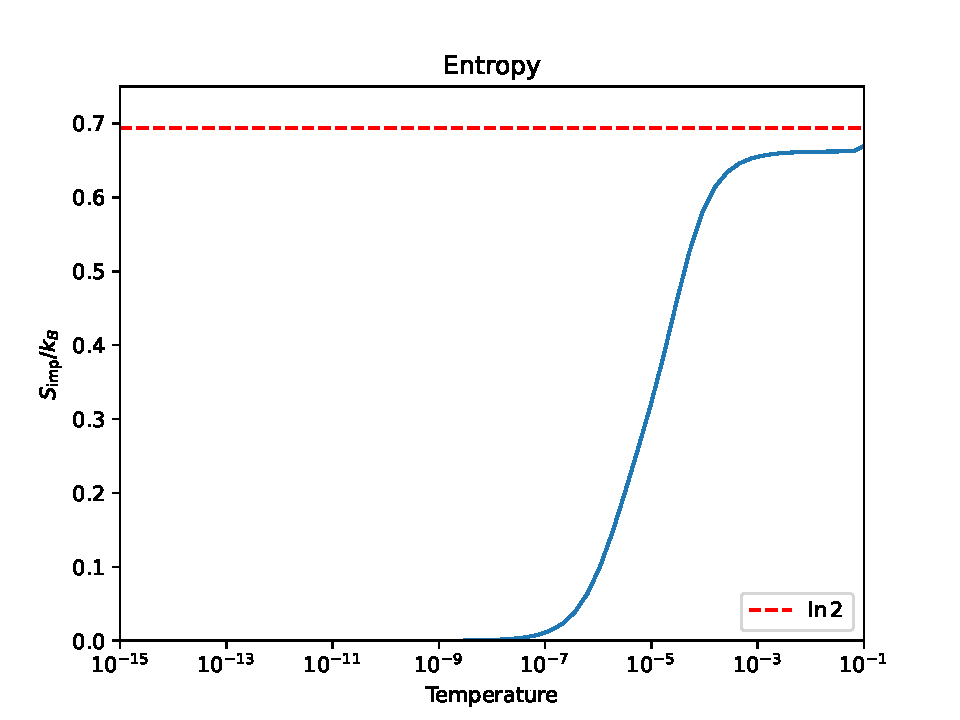
\includegraphics[width=0.65\linewidth]{./gfx/s_lowU.pdf}
  \end{figure}
\end{frame}

\begin{frame}
  \frametitle{Impurity Contribution to Entropy}

  \begin{itemize}
  \item As with the susceptibility, the large $U$ case gives us three fixed points; in the weakly-coupled local moment region, the entropy takes on an intermediate value.
  \end{itemize}

  \begin{figure}
    \centering
    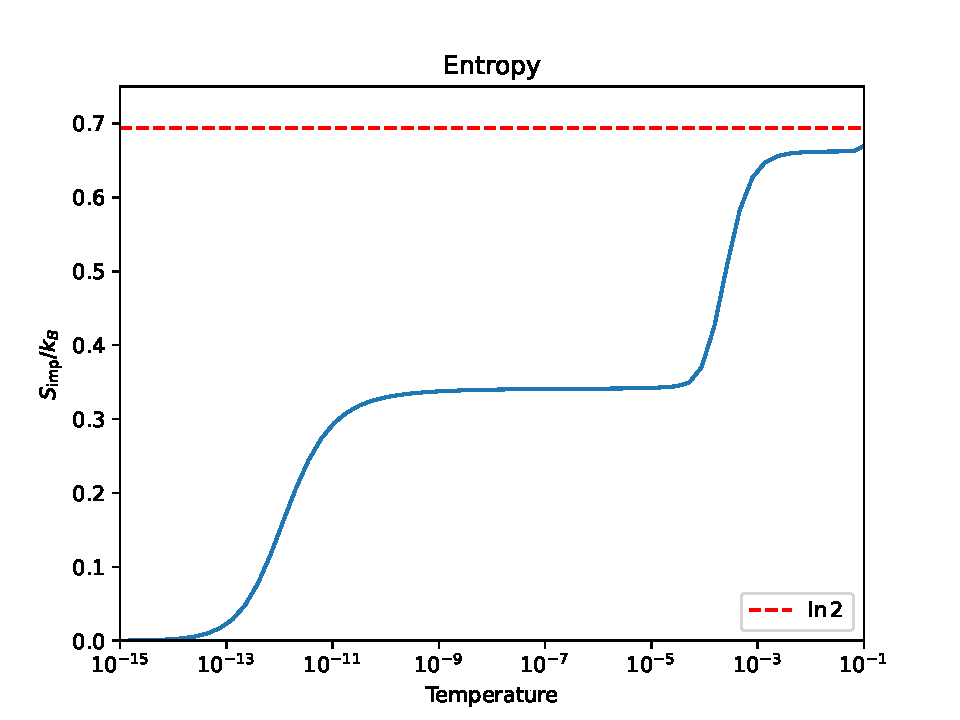
\includegraphics[width=0.65\linewidth]{./gfx/s.pdf}
  \end{figure}
\end{frame}


\begin{frame}
  \frametitle{Impurity Contribution to Specific Heat}

  \begin{itemize}
  \item In both $U$ limits, the impurity's contribution to the specific heat vanishes for $T \ll T_K$ and $T \gg T_K$.
  \item Due to the increased density of states at $T_K$, there is also a peak here in the specific heat, with a second occuring in the large $U$ limit.
  \end{itemize}
  
  \begin{figure}
    \centering
    \includegraphics<1>[width=0.65\linewidth]{./gfx/Cv_lowU.pdf}
    \includegraphics<2>[width=0.65\linewidth]{./gfx/Cv.pdf}
  \end{figure}
\end{frame}

\begin{frame}
  \frametitle{Conclusions}

  \pause 
  \begin{center}
    {\huge The Kondo problem and the NRG are hard!}
  \end{center}
\end{frame}

\begin{frame}
  \frametitle{Conclusions}

  \begin{itemize}
  \item The Kondo problem was a good start at describing magnetic impurities.
  \item Variational/scaling methods helped reveal the qualitative behavior behind the phenomena, namely the formation of a strongly-bound Kondo singlet.
  \item The singlet led to an increased scattering probability within the metal, leading to the observed increase in low-temperature resistivity.
  \item The NRG was the first method that found success due to its non-perturbative nature and finally yielded accurate behavior at temperatures lower than the Kondo temperature.
  \end{itemize}
\end{frame}

\begin{frame}
  \frametitle{References}

  \printbibliography
\end{frame}

\begin{frame}
  \frametitle{Backup}

  \begin{center}
    {\Huge Backup }
  \end{center}
\end{frame}




\begin{frame}
  \frametitle{Logarithmic Discretization}

  \begin{itemize}
  \item The hybrization term looks like:
    \begin{align}
      \int_{-1}^1 \dd\epsilon \; h(\epsilon) f^\dagger_\sigma a_{\epsilon,\sigma} = f^\dagger_\sigma \sum_{np} \Big[ &a_{np\sigma} \int_{x_{n+1}}^{x_n} \dd\epsilon \; h(\epsilon) \psi^+_{np}(\epsilon) \\
                                                                                                                     &+ b_{np\sigma} \int_{-x_n}^{-x_{n+1}} \dd\epsilon \; h(\epsilon) \psi^-_{np}(\epsilon).
    \end{align}
  \item By definition of $\psi^\pm_{np}(\epsilon)$, if we choose a constant hybridization $h(\epsilon) = h$, the integrals filter out the $p=0$ state only:
    \begin{gather*}
      h\int_{x_{n+1}}^{x_n} \dd\epsilon \; \psi^+_{np}(\epsilon) = h\sqrt{d_n} \delta_{p,0}
    \end{gather*}
  \item This corresponds to the fact that the impurity can only couple to the $p=0$ state, so we drop the $p$ index.
  \end{itemize}
\end{frame}

\begin{frame}
  \frametitle{Logarithmic Discretization}

  \begin{itemize}
  \item Defining a step hybridization $h(\epsilon) = h^\pm_n$ that is the average of $\Delta(\epsilon)$ in each interval, we find
    \begin{gather}
      \int_{-1}^1 \dd\epsilon \; h(\epsilon)f^\dagger_\sigma a_{\epsilon,\sigma} = \frac{1}{\sqrt{\pi}}f^\dagger_\sigma \sum_\sigma (\gamma^+_n a_{n0p} + \gamma^-_n b_{n0p}), \\
      (\gamma^+_n)^2 = \int_{x_{n+1}}^{x_n} \dd\epsilon \; \Delta(\epsilon), \quad (\gamma^-_n)^2 = \int_{-x_n}^{-x_{n+1}} \dd\epsilon \; \Delta(\epsilon)
    \end{gather}
  \item The conduction electron term, with all of this, turns into
    \begin{align}
      \int_{-1}^1 \dd\epsilon \; h(\epsilon) a^\dagger_{\epsilon,\sigma} a_{\epsilon,\sigma} &= \sum_{np} (\xi^+_n a^\dagger_{np\sigma}a_{np\sigma} + \alpha^-_n b^\dagger_{np\sigma}b_{np\sigma}) \\
                                                                                             &+ \sum_{n,p \neq p'} \left[ \alpha^+_n(p,p')a^\dagger_{np\sigma}a_{np'\sigma} - \alpha^-_n(p,p')b^\dagger_{np\sigma}b_{np'\sigma} \right].
    \end{align}
  \end{itemize}
\end{frame}

\begin{frame}
  \frametitle{Logarithmic Discretization}

  \begin{itemize}
  \item The $\alpha$ prefactors are defined like so:
    \begin{gather*}
      \alpha^\pm_n(p,p') = \frac{1 - \Lambda^{-1}}{2 \pi i} \frac{\Lambda^{-n}}{p' - p}\exp\left( \frac{2\pi i(p'-p)}{1 - \Lambda^{-1}} \right).
    \end{gather*}
  \item Before we found that the $p=0$ states are filtered out; here we consider $p \neq 0$ states as a perturbation to the $p=0$ part of the $\alpha$ terms, and drop them, leaving
    \begin{align*}
      H = H_{\mathrm{imp}} &+ \sum_{n,\sigma}(\xi^+_n a^\dagger_{n,\sigma} a_{n,\sigma} + \xi^-_n b^\dagger_{n,\sigma} b_{n,\sigma}) \\
                           &+ \frac{1}{\sqrt{\pi}}\sum_\sigma f^\dagger_\sigma \sum_n (\gamma^+_n a_{n,\sigma} + \gamma^-_n b_{n,\sigma})\\
                           &+ \frac{1}{\sqrt{\pi}}\sum_\sigma \left[ \sum_n(\gamma^+_n a^\dagger_{n,\sigma} + \gamma^-_n b^\dagger_{n,\sigma}) \right] f_\sigma.
    \end{align*}
  \item This is finally the fully logarithmically discretized Hamiltonian.
  \end{itemize}
\end{frame}

\begin{frame}
  \frametitle{Mapping to semi-infinite chain}

  \begin{itemize}
  \item The next step is to map this Hamiltonian onto the semi-infinite chain, i.e. in a tight-binding form, with the impurity placed at one end.
  \item In this picture, the impurity only couples to the first conduction site, represented by creation/annihilation operators $c^{(\dagger)}_{0,\sigma}$, the form of which we can read off from the discretized Hamiltonian:
    \begin{gather*}
      c_{0,\sigma} = \frac{1}{\sqrt{\xi_0}}\sum_n(\gamma^+_n a_{n,\sigma} + \gamma^-_n b_{n,\sigma}),
    \end{gather*}
  \item with
    \begin{gather*}
      \xi_0 = \sum_n \left[ (\gamma^+_n)^2 + (\gamma^-_n)^2 \right] = \int_{-1}^1 \dd\epsilon \; \Delta(\epsilon).
    \end{gather*}
  \end{itemize}

  \begin{figure}
    \centering
    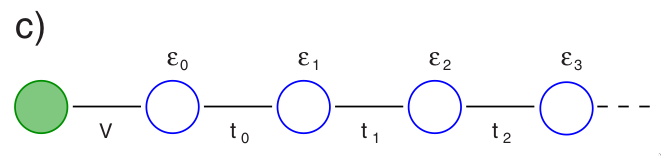
\includegraphics[width=0.5\textwidth]{./gfx/nrg-c.png}
  \end{figure}
\end{frame}



\end{document}

%%% Local Variables:
%%% mode: LaTeX
%%% TeX-master: t
%%% End:

